\section{Creación de Base de Datos}
	\subsection{Caso de Estudio}
	Usted ha sido seleccionado por la empresa TECH TRANSITION para creación de una bodega de datos en
	el departamento de facturación (toda información solicitada en este caso estudio el aprendiz debe
	crearla). Usted debe:
	\begin{itemize}
		\item Elaborar una lista de chequeo con los requerimientos que se deben solucionar.
		\item Verificar si la información está recopilada y organizada actualmente (información que el
		aprendiz debe buscar y/o crear).
		\item Crear una base de datos en Oracle por medio de SQL Developer.
		\item Crear las tablas requeridas en la que defina las siguientes columnas, tipo de datos y relaciones:
			\begin{itemize}
				\item Número de factura.
				\item Fecha de factura.
				\item Fecha de vencimiento.
				\item Cliente.
				\item Sucursal.
				\item Valor total.
				\item Forma de pago.
				\item Valor pagado.
				\item Artículo.
				\item Cantidad.
				\item Valor unitario.
			\end{itemize}
		
	\end{itemize}
	
	\subsection{Lista de Chequeo con los Requerimientos a Solucionar}
	\begin{itemize}
		\item \textbf{Análisis de requerimientos:} Identificar las entidades principales (Factura, Cliente, Sucursal, Artículo).
		\item Auditoría de datos actuales: Evaluar el estado de la información existente en la empresa
		\item \textbf{Configuración del entorno:} Creación del tablespace, usuario (GIBD) y asignación de privilegios en Oracle.
		\item \textbf{Modelado de datos:} Diseño físico de la base de datos definiendo tipos de datos de Oracle (NUMBER, VARCHAR2, DATE)
		\item \textbf{Creación de tablas:} Ejecución de scripts DDL para crear entidades maestras (catálogos).
		\item \textbf{Creación de relaciones:} Implementación de llaves primarias (PK) y foráneas (FK) para garantizar la integridad referencial.
		\item \textbf{Documentación:} Generar la conclusión técnica del caso de estudio.
	\end{itemize}
	
	\subsection{Verificación de la información (Contexto simulado a presentar)}
	Reporte de Estado de la Información (Caso TECH TRANSITION):
	Al iniciar el proyecto, se detectó que la información de facturación no estaba centralizada. Los registros se manejaban en múltiples hojas de cálculo de Excel separadas por sucursal, lo que generaba duplicidad de datos en clientes y artículos, así como errores de digitación en los valores totales. No existía integridad referencial, por lo que un mismo cliente podía tener varios nombres distintos. La información ha sido depurada, clasificada y está lista para ser migrada al nuevo esquema relacional en Oracle, el cual centralizará la operación y evitará anomalías de inserción o actualización

    \subsection{Primera Configuración}
    Se debe crear un usuario diferente a los predeterminados del sistema destinado a gestionar la bodega de datos solicitada en el caso de estudio, para ello ejecutamos la siguiente sentencia en SQL Developer:
    \begin{lstlisting}[language=sql, caption={Creación de Usuario de la Base de Datos}]	
    	-- Creación del usuario y contraseña
    	CREATE USER GIBD IDENTIFIED BY GibdSena2026;
    	-- Asignación de permisos
    	GRANT CREATE SESSION,
    		CREATE TABLE,
    		CREATE VIEW,
    		CREATE SEQUENCE,
    		CREATE PROCEDURE
    	TO GIBD;
    	ALTER USER GIBD QUOTA UNLIMITED ON USERS;
    \end{lstlisting}
    
    \begin{figure}[htbp]
    	\centering
    	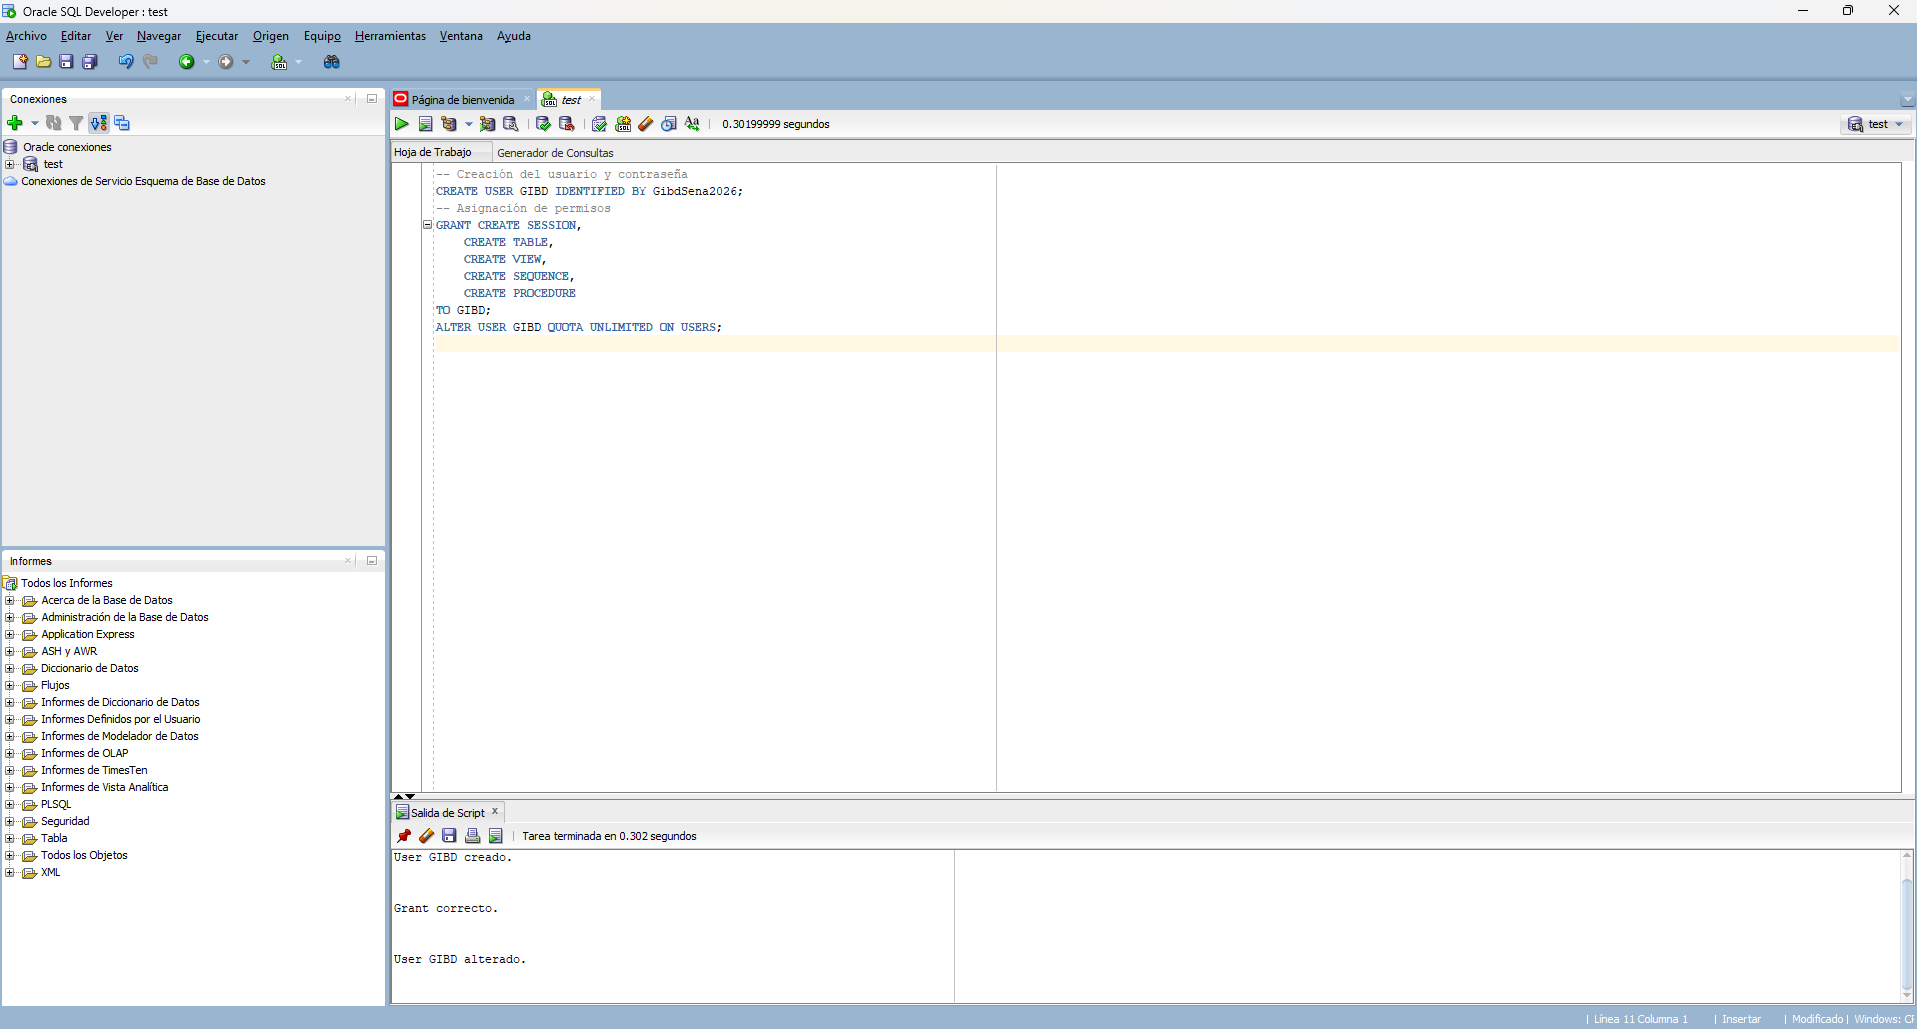
\includegraphics[width=1.0\textwidth]{../../images/dbcreation01.png}
    	\caption{Creación de Usuario nuevo}
    	\label{fig:Creación de nuevo usuario}
    \end{figure}
    \FloatBarrier
    
    \begin{figure}[htbp]
    	\centering
    	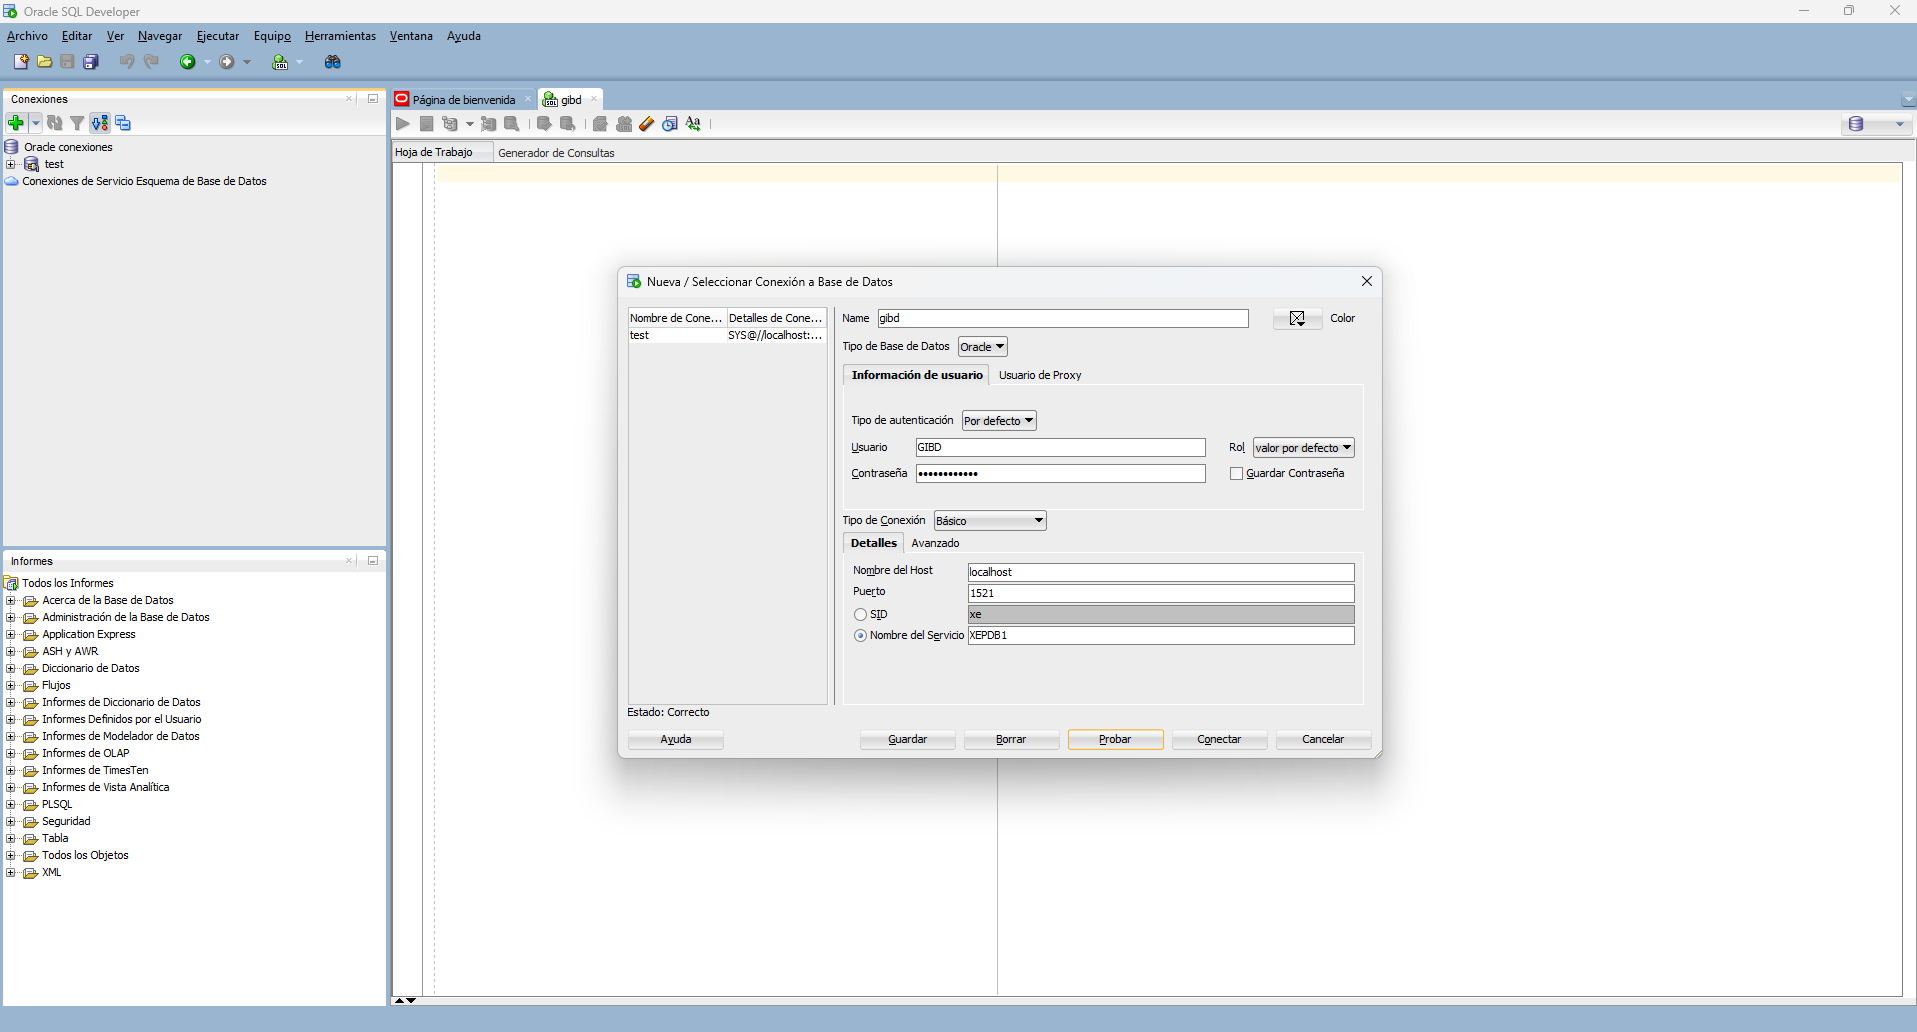
\includegraphics[width=1.0\textwidth]{../../images/dbcreation02.png}
    	\caption{Conexión con Usuario nuevo}
    	\label{fig:Conexión de nuevo usuario}
    \end{figure}
    \FloatBarrier
    
    \subsection{Operaciones DDL para Creación de Tablas y Relaciones}
    Los comandos del Lenguaje de Definición de Datos (DDL) me permiten definir y gestionar un esquema en SQL. En pocas palabras, un esquema en SQL es un plano que define cómo se organizan los datos en una base de datos y cómo se gestionan las relaciones entre las distintas tablas de la base de datos.
    
    \begin{lstlisting}[language=sql, caption={Creación de la base de datos}]	
    	-- 1. TABLAS MAESTRAS (Dimensiones o Catálogos)
    	
    	CREATE TABLE CLIENTES (
    	id_cliente NUMBER GENERATED ALWAYS AS IDENTITY PRIMARY KEY,
    	nombre_cliente VARCHAR2(100) NOT NULL
    	);
    	
    	CREATE TABLE SUCURSALES (
    	id_sucursal NUMBER GENERATED ALWAYS AS IDENTITY PRIMARY KEY,
    	nombre_sucursal VARCHAR2(100) NOT NULL
    	);
    	
    	CREATE TABLE ARTICULOS (
    	id_articulo NUMBER GENERATED ALWAYS AS IDENTITY PRIMARY KEY,
    	nombre_articulo VARCHAR2(100) NOT NULL,
    	valor_unitario_actual NUMBER(10,2) NOT NULL
    	);
    	
    	-- 2. TABLA TRANSACCIONAL PRINCIPAL (Cabecera de Factura)
    	
    	CREATE TABLE FACTURAS (
    	numero_factura NUMBER PRIMARY KEY,
    	fecha_factura DATE NOT NULL,
    	fecha_vencimiento DATE NOT NULL,
    	id_cliente NUMBER NOT NULL,
    	id_sucursal NUMBER NOT NULL,
    	forma_pago VARCHAR2(50) NOT NULL,
    	valor_total NUMBER(12,2) NOT NULL,
    	valor_pagado NUMBER(12,2) NOT NULL,
    	-- Relaciones
    	CONSTRAINT fk_factura_cliente FOREIGN KEY (id_cliente) REFERENCES CLIENTES(id_cliente),
    	CONSTRAINT fk_factura_sucursal FOREIGN KEY (id_sucursal) REFERENCES SUCURSALES(id_sucursal)
    	);
    	
    	-- 3. TABLA TRANSACCIONAL DE DETALLE (Cuerpo de la Factura)
    	
    	CREATE TABLE DETALLE_FACTURAS (
    	numero_factura NUMBER NOT NULL,
    	id_articulo NUMBER NOT NULL,
    	cantidad NUMBER NOT NULL,
    	-- Se guarda el valor unitario en el momento de la venta por si el precio cambia en el futuro
    	valor_unitario NUMBER(10,2) NOT NULL, 
    	-- Llave primaria compuesta
    	PRIMARY KEY (numero_factura, id_articulo),
    	-- Relaciones
    	CONSTRAINT fk_detalle_factura FOREIGN KEY (numero_factura) REFERENCES FACTURAS(numero_factura),
    	CONSTRAINT fk_detalle_articulo FOREIGN KEY (id_articulo) REFERENCES ARTICULOS(id_articulo)
    	);
    \end{lstlisting}
    
    \begin{figure}[htbp]
    	\centering
    	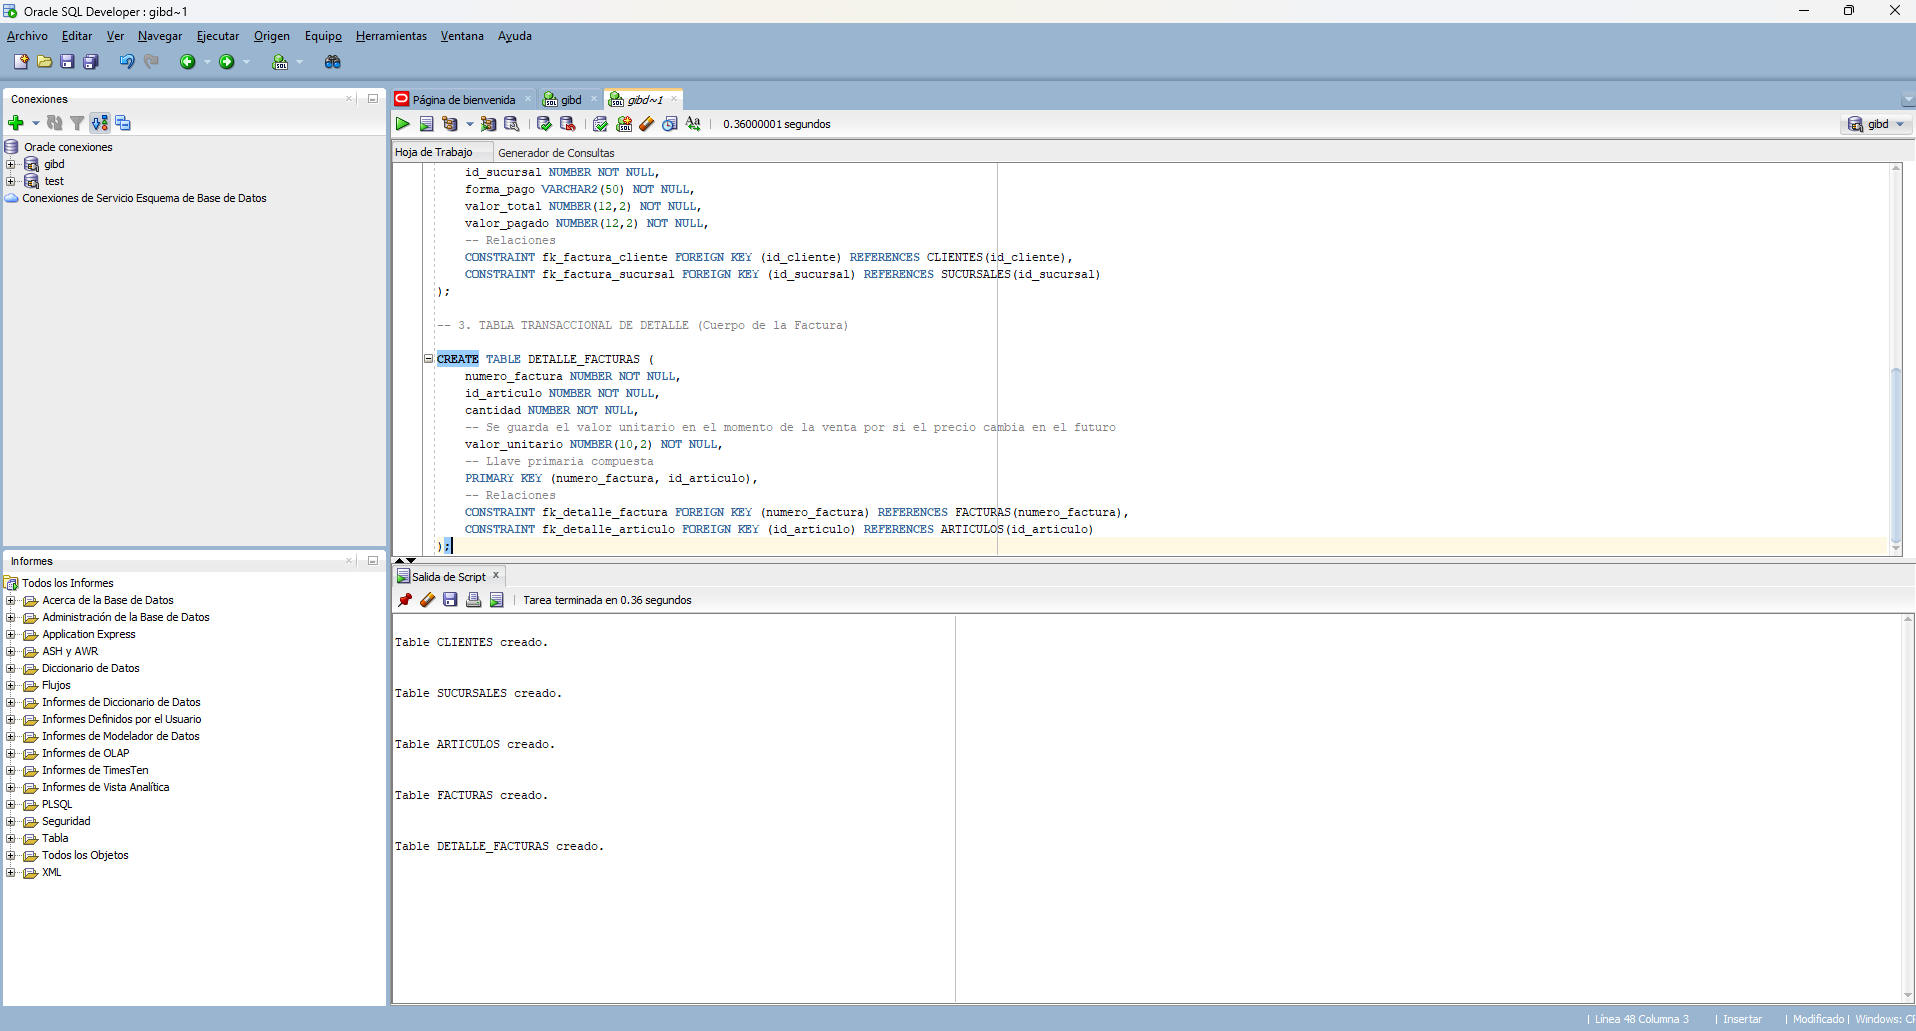
\includegraphics[width=1.0\textwidth]{../../images/dbcreation03.png}
    	\caption{Creación de base datos}
    	\label{fig: Creación de base de datos}
    \end{figure}
    \FloatBarrier